\section{Hagan Rowlenstino/1174040}
	\subsection{Soal 1}
	library matplotlib adalah sebuah library untuk memplotting 2 Dimensi yang output nya adalah gambar publikasi yang bermutu di banyak format hardocpy serta lingkungan interaktif berbagai platform

	\subsection{Soal 2}
	untuk membuat sumbu x dan y :
	\lstinputlisting{src/6/1174040/Teori/chap6_1174040_2.py}

	\subsection{Soal 3}
	\begin{itemize}
		\item PLot Garis :

		\lstinputlisting[firstline=8, lastline=13]{src/6/1174040/Teori/chap6_1174040_3.py}

		\item Plot Sebaran

		\lstinputlisting[firstline=15, lastline=18]{src/6/1174040/Teori/chap6_1174040_3.py}

		\item Plot Batang / Histogram

		\lstinputlisting[firstline=20, lastline=23]{src/6/1174040/Teori/chap6_1174040_3.py}

		\item Pie

		\lstinputlisting[firstline=26, lastline=35]{src/6/1174040/Teori/chap6_1174040_3.py}

	\end{itemize}

	\subsection{Soal 4}
	\begin{itemize}
		\item Legend : Penjelasan garis beserta contoh dari garis yang dijelaskan tersebut. untuk membuat legend dapat menggunakan sintaks berikut :

		\begin{verbatim} legend('legend grafik1',…,'legend grafikN','Nilai Pos') \end{verbatim}
		
		\item Label : Memberikan penamaan untuk skala(sumbu) yang kita buat. untuk menambahkan label, kita dapat menggunakan sintaks berikut :

		\begin{verbatim} 
		xlabel(‘teks horizontal axis’)

		ylabel(‘teks vertikal axis’)
		\end{verbatim}
	\end{itemize}

	\subsection {Soal 5}
	Subplot pada matplotlib berfungsi untuk membuat banyak plot grafik dalam satu figure saja.
	dimana  subplot dapat kita definisikan sebagai berikut :
	
	\begin{verbatim} subplot(m,n,i) 
	\end{verbatim}
	Dimana m adalah tinggi nya, n adalah lebar nya dan i adalah urutan penempatannya.
	Untuk membuat 9 subplot dapat dilihati dari contoh dibawah ini :

	\lstinputlisting{src/6/1174040/Teori/chap6_1174040_5.py}

	\begin{figure}[ht]
            \centerline{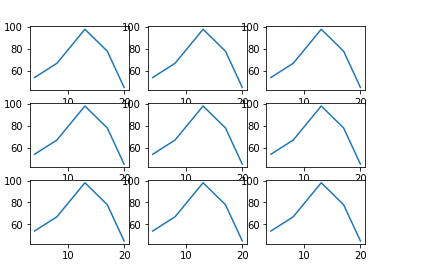
\includegraphics[width=0.5\textwidth]{figures/6/1174040/Teori/1174040_no5.png}}
            \caption{No. 5}
            \label{1174040_chap6_no5}
            \end{figure}

	\subsection{Soal 6}
	color yang dapat digunakan adalah red(r),blue(b),green(g),cyan(c),magenta(m),yellow(y),black(k),white(w)

	\subsection{Soal 7}
	fungsi Hist digunakan untuk membuat histogram yang berfungsi untuk menampilkan frekuensi data dengan menggunakan grafik batang

	\lstinputlisting{src/6/1174040/Teori/chap6_1174040_hist.py}

	\begin{figure}[ht]
            \centerline{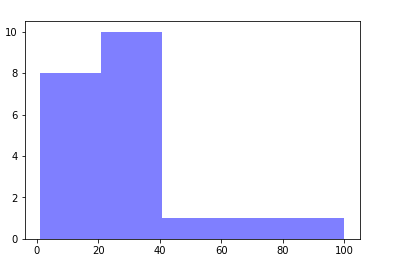
\includegraphics[width=0.5\textwidth]{figures/6/1174040/Teori/1174040_no7.png}}
            \caption{No. 7}
            \label{1174040_chap6_no7}
            \end{figure}

	\subsection{Soal 8}
	\begin{itemize}
		\item Labels : Untuk memberi penamaan terhadap setiap potongan dari pie
		\item colors : Untuk memberikan warna spesifik terhadap potongan potongan pie, jika tidak diberi warna maka dia akan menggambi warna dari pie yang telah berjalan
		\item startangle : Untuk menetapkan dari sudut mana grafik tersebut akan dimulai
		\item shadow : untuk memberikan efek bayangan di bawah pie maupun potongannya
		\item explode : untuk menentukan seerapa jauh pemisahkan potongan pie dari potongan - potongan lainnya
		\item autopct : untuk memberikan nilai atau skalal numeric pada label didalam potongan pie . seperti mengubah dari 10 menjadi 10.0
	\end{itemize}

	\subsection{Cek Plagiarisme}
	
	\begin{figure}[ht]
            \centerline{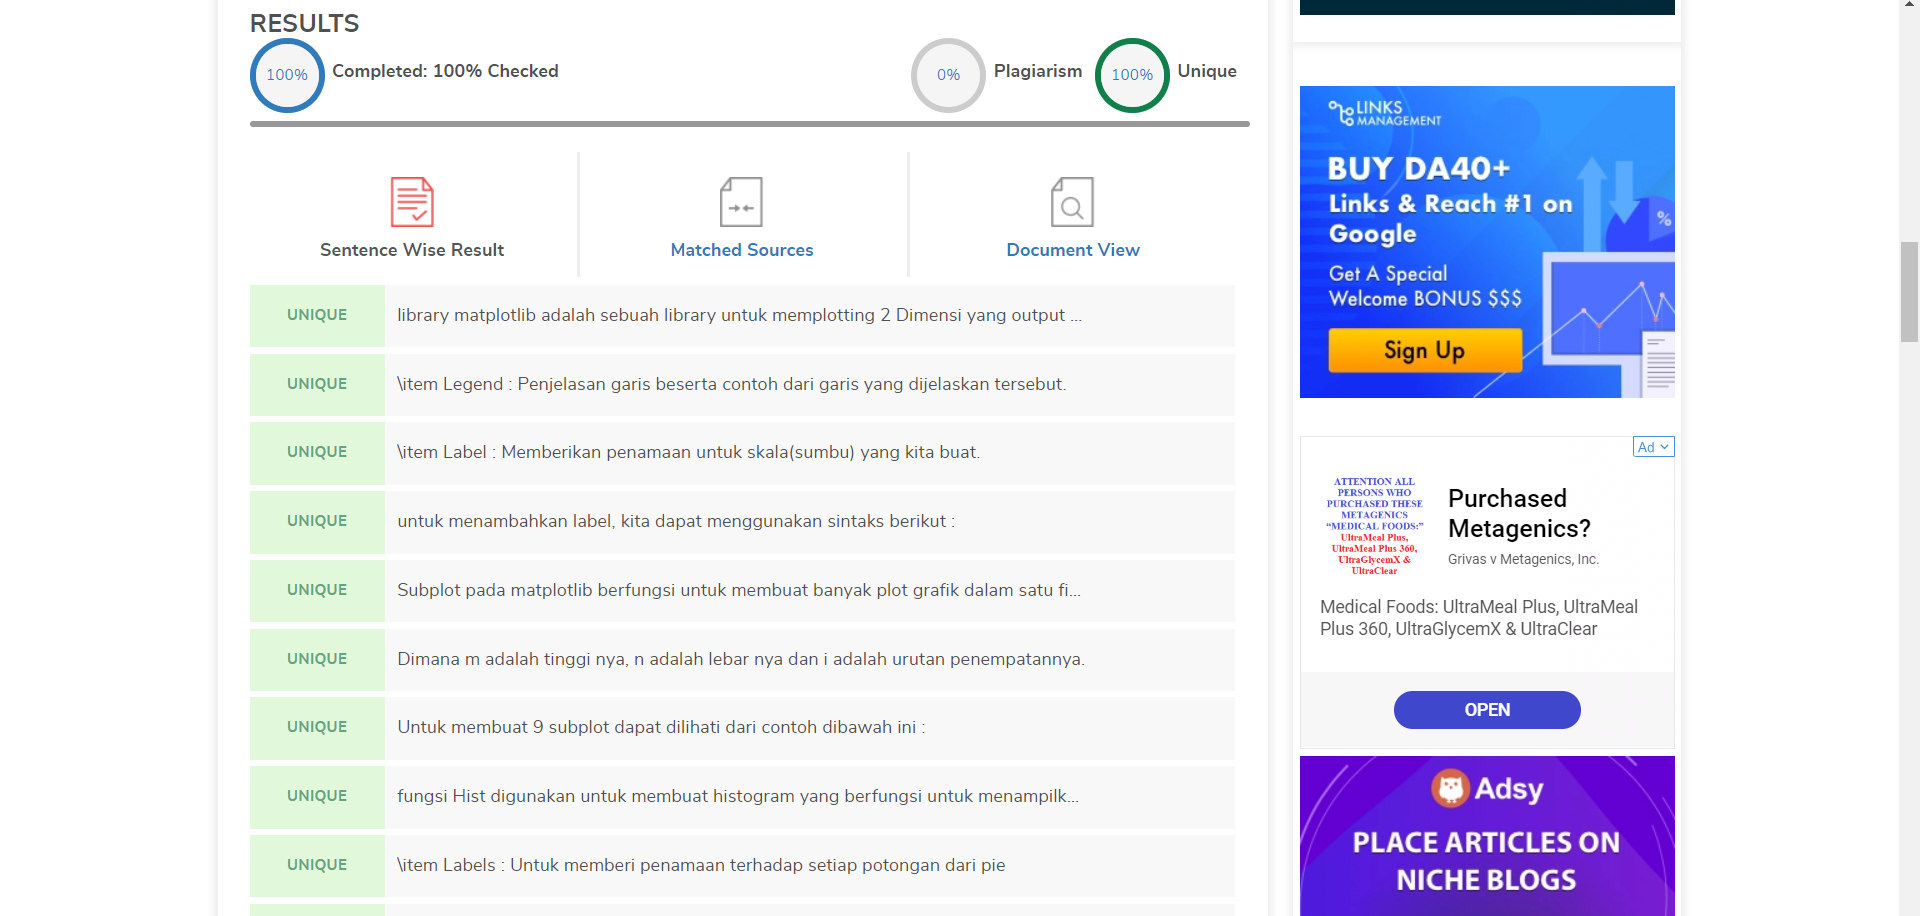
\includegraphics[width=0.5\textwidth]{figures/6/1174040/Teori/1174040_plagiat.png}}
            \caption{Cek Plagiarisme}
            \label{1174040_chap6_plagiat}
            \end{figure}
			
\section{Irvan Rizkiansyah/1174043}
	\subsection{Nomor 1}
		matplotlib merupakan library plotting 2D Python dan berfungsi untuk membuat plot, histogram, grafik batang, scatterplot, dan masih banyak yang lainnya hanya dengan beberapa baris code saja.
		
	\subsection{Nomor 2}
	Pembuatan sumbu X dan Y di matplotlib, mirip dengan membuat sebuah variabel yang mempunyai array. Kemudian variabel yang dibuat yang nanti-nya akan menjadi sumbu X dan Y dan akan dipanggil menggunakan fungsi plot.
		\lstinputlisting[firstline=8, lastline=14]{src/6/1174043/Teori/chap6_1174043_no2.py}
	
	\subsection{Nomor 3}
	Perbedaan fungsi yang ada pada matplotlib :
		\begin{itemize}
			\item Fungsi scatter atau plot sebaran merupakan sebuah grafik yang menunjukkan hubungan dari dua set data, seperti halnya hubungan dari tinggi badan dan berat badan.
			Cara menggunakannya dengan memanggil fungsi scatter yang terdapat pada matplotlib \begin{verbatim} matplotlib.pyplot.scatter(x,y) \end{verbatim}
			
			\item Fungsi histogram merupakan sebuah grafik yang akan menampilkan frekuensi data menggunakan sebuah batang.
			Cara menggunakannya dengan memanggil fungsi hist yang terdapat pada matplotlb \begin{verbatim} matplotlib.pyplot.hist(x,y) \end{verbatim}
			
			\item Fungsi plot garis atau plot sinus merupakan sebuah grafik yang menunjukkan frekuensi data menggunakan garis.
			Cara menggunakannya dengan memanggil fungsi plot yang terdapat pada matplotlib \begin{verbatim} matplotlib.pyplot.plot(x,y) \end{verbatim}
			
		\end{itemize}
	Dan masih banyak yang lainnya.
	\subsection{Nomor 4}
	Fungsi legend merupakan dimana akan menamai sebuah bar pada grafik untuk membedakan bar tersebut dengan bar yang lainnya, dimana jika terdapat banyak bar pada grafik tersebut. Sedangkan fungsi label untuk menamai sumbu x dan sumbu y.
	Cara menggunakannya hanya tinggal memanggil fungsi legend dan fungsi label yang terdapat pada matplotlib dan memberikan nama untuk legend dan label tersebut. Contohnya :
		\lstinputlisting[firstline=8, lastline=19]{src/6/1174043/Teori/chap6_1174043_legend.py}
	
	\subsection{Nomor 5}
	Fungsi subplot adalah untuk memanggil banyak grafik hanyak dengan sekali panggil saja. Cara kerja dari fungsi subplot ini sendiri cukup simpel, dimana cukup memanggil fungsi subplot yang terdapat pada matplotlib 
	\begin{verbatim} matplotlib.pyplot.subplot(nbaris, nkolom, index) \end{verbatim}
	Dibawah ini merupakan ilustrasi dan parameter apa saja yang digunakan jika ingin menggambar plot dengan 9 sub plot :
		\lstinputlisting[firstline=8, lastline=54]{src/6/1174043/Teori/chap6_1174043_subplot.py}
		
	\subsection{Nomor 6}
	Matplotlib mengenal beberapa format untuk color diantaranya :
		\begin{itemize}
			\item RGB atau RGBA contohnya (0.1, 0.2, 0.5)
			\item hex RGB atau RGBA contohnya '\#0F0F0F
			\item Representasi string dari nilai float contohnya '0.5'
			\item atau hanya seperti kata awal dari warna tersebut yang ingin digunakan contohnya warna Cyan maka hanya perlu menggunakan 'c', warna Green maka hanya perlu menggunakan 'g' dan masih banyak yang lainnya seperti 'b', 'r', 'm', dan yang lainnya
			\item X11/CSS4 nama warna
			\item nama dari xkcd color survey contohnya 'xkcd:sky blue'
			\item Tableau Color dari 'T10' pallette kategorikal contohnya 'tab:olive'
			
		\end{itemize}
	
	\subsection{Nomor 7}
	Fungsi hist merupakan fungsi untuk menggunakan grafik bar atau batang, dimana frekuensi setiap elemen data yang ada pada daftar ditunjukkan dengan grafik histogram. Angka yang dikelompokkan dalam bentuk rentang tertentu yang sudah di tentukan dsebut bins.
		\lstinputlisting[firstline=8, lastline=12]{src/6/1174043/Teori/chap6_1174043_histogram.py}
	
	\subsection{Nomor 8}
	Parameter yang terdapat pada fungsi pie :
		\begin{itemize}
			\item labels : dimana berfungsi untuk memberi nama untuk setiap slice yang terdapat pada grafik pie
			\item colors : dimana berfungsi untuk memberikan warna untuk setiap slice yang terdapat pada gradik pie
			\item startangle : dimana berfungsi jika tidak tidak ada, maka awalan putaran dari grafik pie berlawanan dari arah jarum jam dari titik sumbu x
			\item shadow : dimana berfungsi untuk memberikan efek grafis bayangan pada grafik pie
			\item explode : dimana berfungsi untuk menentukan fraksi dari jari-jari untuk mengimbangi setiap slice menggunakan sumbu x
			\item autopct : string atau fungsi yang digunakan untuk label pada slice dengan nilai numerik, maka label akan ditempatkan didalam slice.			
		\end{itemize}

\section{Luthfi Muhammad Nabil/1174035}
\subsection{Soal 1}
Apa itu fungsi library matplotlib

Library matplotlib adalah library bahasa pemrograman python untuk menampilkan grafik - grafik sehingga data dapat divisualisasikan dengan lebih baik. Isi dari grafik tersebut dapat menggunakan data sesuai kebutuhan. Matplotlib sudah digunakan banyak aplikasi data sains untuk menampilkan visualisasi data yang berupa grafik. 

\subsection{Soal 2}
Jelaskan langkah-langkah membuat sumbu X dan Y di matplotlib

Pada library matplotlib, hanya membutuhkan dua variabel atau dua kumpulan data yang memiliki posisi sama. Isi dari data tersebut menggunakan nilai angka dan isinya dapat berupa integer atau float. Berikut contoh dari koding menampilkan data dengan sumbu X dan Y : 
\lstinputlisting[firstline=2, lastline=6]{src/6/1174035/Teori/chap6_1174035_Teori.py}
Berikut hasilnya terdapat pada gambar \ref{Contoh_Soal2}
\begin{figure} [ht]
	\centerline{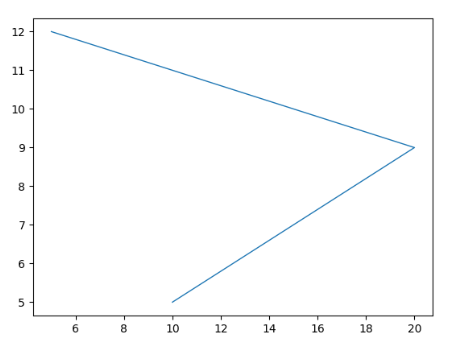
\includegraphics[width=0.6\textwidth]{figures/6/1174035/Teori/Soal2.png}}
	\caption{Contoh Pengaplikasian Sumbu X dan Y}
	\label{Contoh_Soal2}
\end{figure}

\subsection{Soal 3}
Jelaskan bagaimana perbedaan fungsi dan cara pakai untuk berbagai jenis plot di matplotlib
\begin{itemize}
	\item Grafik Garis
	
	Untuk plot pada diagram garis, dibutuhkan data nilai angka yang dapat berupa satu atau dua kumpulan data. Berikut pengaplikasian untuk diagram garis : 
	\lstinputlisting[firstline=9, lastline=12]{src/6/1174035/Teori/chap6_1174035_Teori.py}
	Atau dapat juga mengubah jalur garis dengan 2 kumpulan angka seperti berikut : 
	\lstinputlisting[firstline=15, lastline=18]{src/6/1174035/Teori/chap6_1174035_Teori.py}
	\begin{figure} [ht]
		\centerline{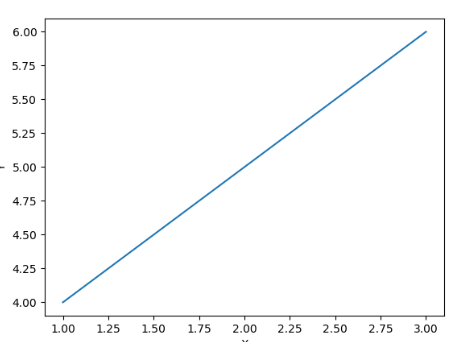
\includegraphics[width=0.6\textwidth]{figures/6/1174035/Teori/Soal3Garis.png}}
		\caption{Contoh Grafik Garis}
		\label{Contoh_Soal3Garis}
	\end{figure}
	
	\item Grafik Titik
	
	Untuk plot pada diagram titik, dapat melakukan langkah seperti berikut : 
	\lstinputlisting[firstline=21, lastline=26]{src/6/1174035/Teori/chap6_1174035_Teori.py}
	Terlihat perbedaannya pada penambahan parameter ketiga dengan isinya yaitu 'ro'
	\begin{figure} [ht]
		\centerline{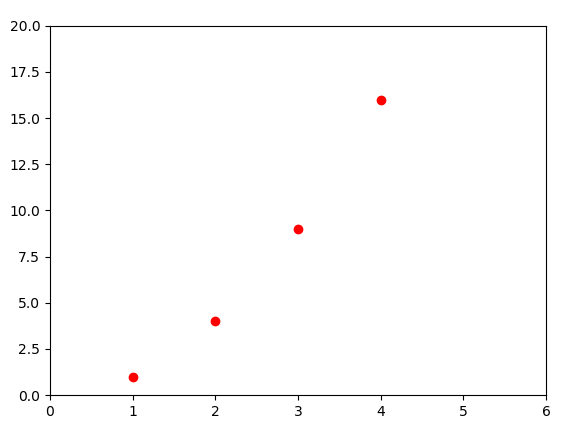
\includegraphics[width=0.6\textwidth]{figures/6/1174035/Teori/Soal3Titik.png}}
		\caption{Contoh Grafik Titik}
		\label{Contoh_Soal3Titik}
	\end{figure}
	
	\item Grafik Batang
	
	Untuk plot diagram batang diperlukan koding baru menggunakan plt.bar(). Contoh pengaplikasian dapat diaplikasikan sebagai berikut : 
	\lstinputlisting[firstline=29, lastline=31]{src/6/1174035/Teori/chap6_1174035_Teori.py}
	Hasil dapat dilihat pada gambar \ref{Contoh_Soal3Batang}
	\begin{figure} [ht]
		\centerline{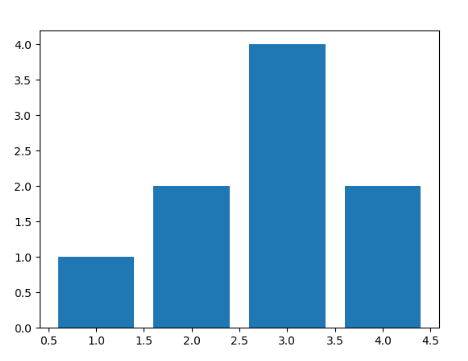
\includegraphics[width=0.6\textwidth]{figures/6/1174035/Teori/Soal3Batang.png}}
		\caption{Contoh Grafik Batang}
		\label{Contoh_Soal3Batang}
	\end{figure}
	
	\item Grafik Lingkaran
	
	Untuk plot diagram batang perlu menggunakan subplot. Berikut contoh pengaplikasiannya : 
	\lstinputlisting[firstline=34, lastline=43]{src/6/1174035/Teori/chap6_1174035_Teori.py}
	Hasil dapat dilihat pada gambar \ref{Contoh_Soal3Pie}
	\begin{figure} [ht]
		\centerline{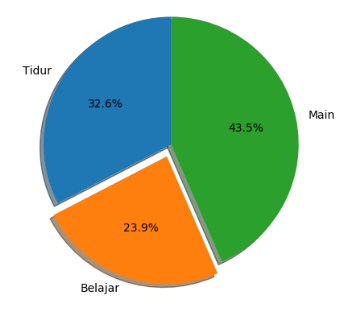
\includegraphics[width=0.6\textwidth]{figures/6/1174035/Teori/Soal3Pie.png}}
		\caption{Contoh Grafik Pie}
		\label{Contoh_Soal3Pie}
	\end{figure}
\end{itemize}

\subsection{Soal 4}
Jelaskan bagaimana cara menggunakan legend dan label serta kaitannya dengan fungsi tersebut
\begin{itemize}
\item Label

Untuk menggunakan label, hanya perlu menambahkan sintaks plt.xlabel() atau plt.ylabel(). Label berfungsi untuk memberikan label pada setiap garis atau label untuk gambar yang ada. Berikut contoh untuk menambahkan label pada matplotlib : 
\lstinputlisting[firstline=46, lastline=52]{src/6/1174035/Teori/chap6_1174035_Teori.py}
Pada sintaks berikut, akan menambahkan label pada sumbu x dengan tulisan 'X', begitu juga dengan sumbu y dengan label 'Y'. Berikut hasilnya pada gambar \ref{Contoh_Soal4Label} 
\begin{figure} [ht]
	\centerline{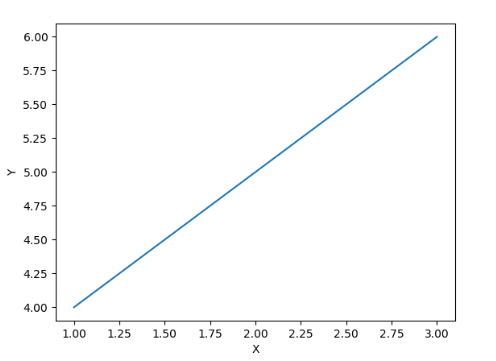
\includegraphics[width=0.6\textwidth]{figures/6/1174035/Teori/Soal4Label.png}}
	\caption{Contoh Pengaplikasian Label}
	\label{Contoh_Soal4Label}
\end{figure}

\item Legend

Untuk menggunakan legend, perlu mengadakan label saat menginisiasi sebuah plot. Berikut contoh penggunaan legend : 
\lstinputlisting[firstline=54, lastline=59]{src/6/1174035/Teori/chap6_1174035_Teori.py}

Pada sintaks plt.plot(), terdapat parameter untuk menginput label yang isinya 'Garis Satu' untuk mengatur isi atau judul dari label tersebut. Lalu plt.legend() adalah sintaks untuk menunjukan legend yang akan dimunculkan. Berikut contoh dari pengaplikasiannya pada gambar \ref{Contoh_Soal4Legend} 
\begin{figure} [ht]
	\centerline{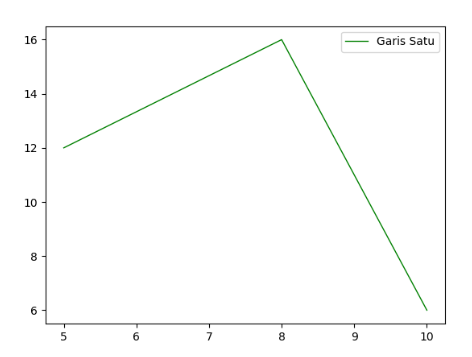
\includegraphics[width=0.6\textwidth]{figures/6/1174035/Teori/Soal4Legend.png}}
	\caption{Contoh Pengaplikasian Legend}
	\label{Contoh_Soal4Legend}
\end{figure}
\end{itemize}

\subsection{Soal 5}
Jelaskan apa fungsi dari subplot di matplotlib, dan bagaimana cara kerja dari fungsi subplot

Subplot adalah fungsi untuk menampilkan beberapa diagram pada satu aplikasi atua sintaks. Untuk menginisiasi subplot, dapat menggunakan fungsi plt.subplot() dan memasukan ukuran subplot di dalamnya (Contoh : plt.subplot(331)). Pada fungsi plt.subplot(331), angka pertama pada contoh merupakan jumlah baris yang dapat dipakai dan angka kedua merupakan jumlah kolom yang dapat dipakai sedangkan angka ketiga merupakan di baris dan kolom berapa grafik akan disimpan. Posisi grafik dimulai dari kiri atas dan berpindah ke kanan dan jika sudah mencapai batas kolom maka akan berpindah ke baris selanjutnya yang dimulai dari kiri kembali. Contoh penggunaan subplot : 
\lstinputlisting[firstline=61, lastline=103]{src/6/1174035/Teori/chap6_1174035_Teori.py}
Berikut hasil yang didapat pada koding berikut ditampilkan pada gambar \ref{Contoh_Soal5}
\begin{figure} [ht]
	\centerline{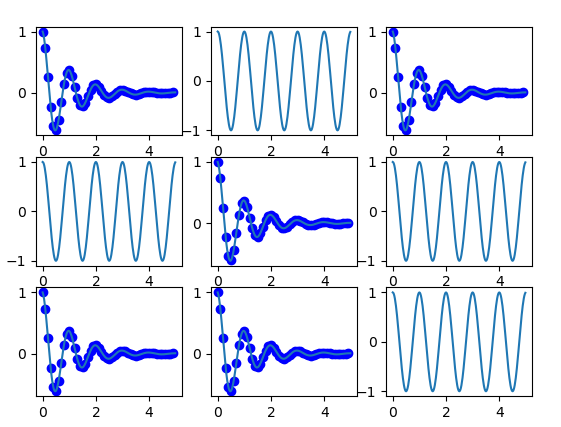
\includegraphics[width=0.6\textwidth]{figures/6/1174035/Teori/Soal5.png}}
	\caption{Contoh Pengaplikasian Subplot}
	\label{Contoh_Soal5}
\end{figure}

\subsection{Soal 6}
Sebutkan semua parameter color yang bisa digunakan

\begin{itemize}
	\item b : Untuk memberikan warna biru
	\item g : Untuk memberikan warna hijau
	\item r : Untuk memberikan warna merah
	\item c : Untuk memberikan warna biru muda
	\item m : Untuk memberikan warna pink
	\item y : Untuk memberikan warna kuning
	\item k : Untuk memberikan warna hitam
	\item w : Untuk memberikan warna putih
\end{itemize}

\subsection{Soal 7}
Jelaskan bagaimana cara kerja dari fungsi hist

Fungsi hist pada library matplotlib yaitu menhistorgramkan kumpulan data yang akan ditampilkan biasanya berupa grafik batang. Grafik akan dimasukkan beberapa data dan diambil frekuensi dari data tersebut. Berikut contoh koding dari histogram : 
\lstinputlisting[firstline=106, lastline=113]{src/6/1174035/Teori/chap6_1174035_Teori.py}
Berikut hasil dari histogram yang ada pada gambar \ref{Contoh_Soal7}
\begin{figure} [ht]
	\centerline{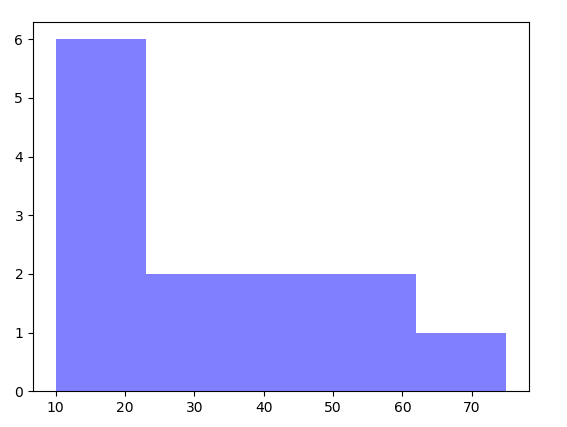
\includegraphics[width=0.6\textwidth]{figures/6/1174035/Teori/Soal7.png}}
	\caption{Contoh Pengaplikasian Histogram}
	\label{Contoh_Soal7}
\end{figure}
\subsection{Soal 8}
Jelaskan lebih mendalam tentang parameter dari fungsi pie.

\begin{itemize}
	\item labels : Isi dengan tipe data list dan tidak wajib untuk digunakan. Fungsi parameter labels untuk memberi label pada setiap pecahan data yang ada pada grafik pie yang ditampilkan.
	\item colors : Tipe data array atau sejenis dan tidak wajib untuk digunakan. Fungsi parameter colors untuk mengganti warna pada setiap pecahan yang ada. Jika tidak digunakan atau ditentukan, maka warna yang akan dipakai adalah warna yang aktif atau standar.
	\item startangle : Tipe data pecahan atau float, tidak wajib untuk digunakan. Fungsi parameter startangle adalah fungsi untuk memutar grafik agar berubah posisi dengan acuan yaitu angle awalan dari grafik pie.
	\item shadow : Bertipe data boolean dan tidak wajib digunakan. Fungsi parameter shadow digunakan untuk membuat bayangan pada bawah grafik pie yang ditampilkan. 
	\item explode : Bertipe data array atau sejenis dan tidak wajib digunakan. Fungsi parameter explode adalah menentukan radius untuk mengimbangi setiap pecahan pada grafik pie. Jika radius lebih dari 0 maka pecahan akan mulai menjauh dari pusat dan terlihat seperti keluar dari grafik lingkaran tersebut.
	\item autopct : Bertipe data string atau fungsi dan tidak wajib digunakan. Fungsi parameter autopct adalah memberi label pada irisan dengan labelnya berupa fungsi atau string. 
\end{itemize}

\subsection{Plagiarisme}
Berikut hasil pengecekan plagiarisme untuk bagian teori terdapat pada gambar \ref{Plagiarisme}.
\begin{figure} [ht]
	\centerline{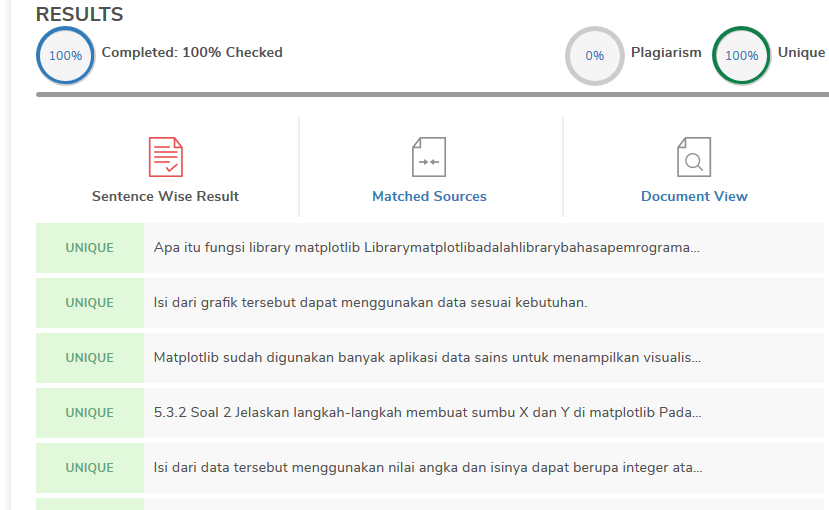
\includegraphics[width=0.6\textwidth]{figures/6/1174035/Teori/Plagiarisme.png}}
	\caption{Cek Plagiarisme}
	\label{Plagiarisme}
\end{figure}


\section{Faisal Najib Abdullah 1174042}
\subsection{Teori}
\subsubsection{Soal No. 1}
\hfill \break
Apa itu fungsi library matplotlib?

\hfill \break
Matplotlib merupakan salah satu library Python 2D yang dapat menghasilkan plot dengan kualitas yang tinggi dalam berbagai format dan dapat digunakan di berbagai platform. Matplotlib berfungsi sebagai pembuat grafik di berbagai platform, seperti Python dan Jupyter. Grafik yang dibuat menggunakan Matplotlib bisa dibuat dalam berbagai bentuk, seperti grafik garis, batang, lingkaran, histogram, dan sebagainya.

\subsubsection{Soal No. 2}
\hfill \break
Jelaskan langkah-langkah membuat sumbu X dan Y di matplotlib!

\begin{enumerate}
	\item Pertama import library Matplotlib.	
	\lstinputlisting[firstline=2, lastline=2]{src/6/1174042/1174042.py}
	
	\item Buat variabel x yang menampung list untuk sumbu x dan variabel y yang menampung list untuk sumbu y.	
	\lstinputlisting[firstline=4, lastline=5]{src/6/1174042/1174042.py}
	
	\item Panggil fungsi plot dan isi parameter pertama dengan variabel x dan parameter kedua dengan variabel y.
	\lstinputlisting[firstline=7, lastline=7]{src/6/1174042/1174042.py}	

	\item Lalu panggil plot tadi dengan memanggil fungsi show.
	\lstinputlisting[firstline=9, lastline=9]{src/6/1174042/1174042.py}
	
\end{enumerate}
\hfill \break
\textbf{Kode Program}

\lstinputlisting[caption = Kode program membuat diagram menggunakan Matplotlib., firstline=2, lastline=9]{src/6/1174042/1174042.py}

\hfill \break
\textbf{Hasil Compile}

\begin{figure}[H]
	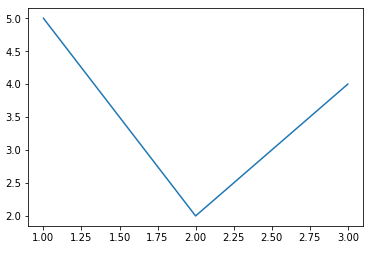
\includegraphics[width=12cm]{figures/6/1174042/1.png}
	\centering
	\caption{Hasil compile membuat diagram menggunakan Matplotlib.}
\end{figure}
 
\subsubsection{Soal No. 3}
\hfill \break
Jelaskan bagaimana perbedaan fungsi dan cara pakai untuk berbagai jenis(bar, histogram ,scatter ,line, dll) jenis plot di matplotlib!

\begin{enumerate}
	\item \textbf{Bar Graph}
	
	Perbedaan bar graph dengan jenis plot yang lain adalah bar graph menggunakan bar atau batang-batang untuk membandingkan data di antara berbagai kategori.
	
	\textbf{Kode Program}
	
	\lstinputlisting[caption = Kode program membuat bar graph menggunakan Matplotlib., firstline=13, lastline=25]{src/6/1174042/1174042.py}
	
	\textbf{Hasil Compile}
	
	\begin{figure}[H]
		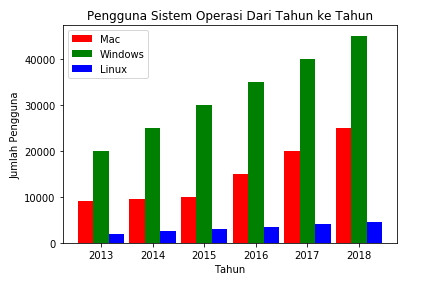
\includegraphics[width=12cm]{figures/6/1174042/2.png}
		\centering
		\caption{Hasil compile membuat bar graph menggunakan Matplotlib.}
	\end{figure}
	
	\item \textbf{Histogram}
	
	Perbedaan histogram dengan jenis plot yang lain adalah histogram akan membuat plot dimana plot yang dimunculkan merupakan gabungan dari beberapa data yang telah dikelompokkan.
	
	\textbf{Kode Program}
	
	\lstinputlisting[caption = Kode program membuat histogram menggunakan Matplotlib., firstline=29, lastline=36]{src/6/1174042/1174042.py}
	
	\textbf{Hasil Compile}
	
	\begin{figure}[H]
		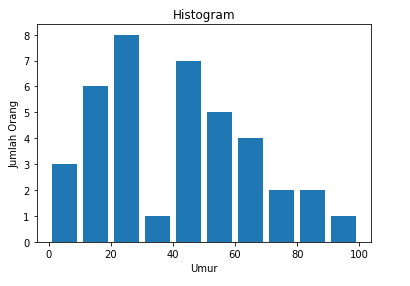
\includegraphics[width=12cm]{figures/6/1174042/3.png}
		\centering
		\caption{Hasil compile membuat histogram menggunakan Matplotlib.}
	\end{figure}
	
	\item \textbf{Scatter Plot}
	
	Perbedaan scatter plot dengan jenis plot lain adalah scatter plot menampilkan data sebagai kumpulan titik, masing-masing memiliki nilai satu variabel yang menentukan posisi pada sumbu horizontal dan nilai variabel lain menentukan posisi pada sumbu vertikal.
	
	\textbf{Kode Program}
	
	\lstinputlisting[caption = Kode program membuat scatter plot menggunakan Matplotlib., firstline=40, lastline=53]{src/6/1174042/1174042.py}
	
	\textbf{Hasil Compile}
	
	\begin{figure}[H]
		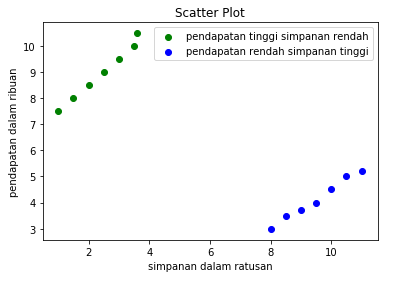
\includegraphics[width=12cm]{figures/6/1174042/4.png}
		\centering
		\caption{Hasil compile membuat scatter plot menggunakan Matplotlib.}
	\end{figure}
	
	\item \textbf{Area Plot}
	
	Perbedaan area plot dengan jenis plot lain adalah area plot digunakan untuk melacak perubahan dari waktu ke waktu untuk dua atau lebih kelompok terkait yang membentuk satu kategori secara keseluruhan.
	
	\textbf{Kode Program}
	
	\lstinputlisting[caption = Kode program membuat diagram menggunakan Matplotlib., firstline=57, lastline=76]{src/6/1174042/1174042.py}
	
	\textbf{Hasil Compile}
	
	\begin{figure}[H]
		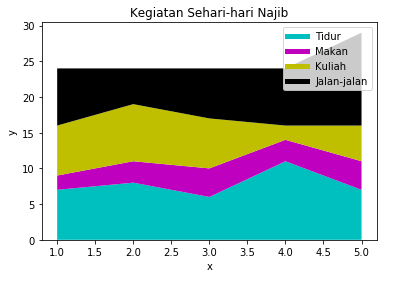
\includegraphics[width=12cm]{figures/6/1174042/5.png}
		\centering
		\caption{Hasil compile membuat diagram menggunakan Matplotlib.}
	\end{figure}
	
	\item \textbf{Pie Plot}
	
	Perbedaan pie plot dengan jenis plot lain adalah pie plot digunakan untuk menunjukkan persentase atau data proporsional di mana setiap potongan pie mewakili kategori.
	
	\textbf{Kode Program}
	
	\lstinputlisting[caption = Kode program membuat Pie Plot menggunakan Matplotlib., firstline=86, lastline=101]{src/6/1174042/1174042.py}
	
	\textbf{Hasil Compile}
	
	\begin{figure}[H]
		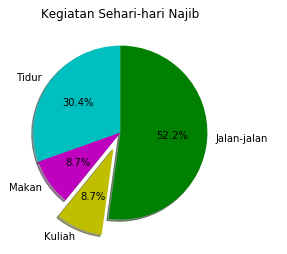
\includegraphics[width=9cm]{figures/6/1174042/6.png}
		\centering
		\caption{Hasil compile membuat Pie Plot menggunakan Matplotlib.}
	\end{figure}
	
	\item \textbf{Line Graph}
	
	Perbedaan line graph dengan jenis plot lain adalah line graph menampilkan diagram dalam bentuk garis.
	
	\textbf{Kode Program}
	
	\lstinputlisting[caption = Kode program membuat diagram menggunakan Matplotlib., firstline=105, lastline=113]{src/6/1174042/1174042.py}
	
	\textbf{Hasil Compile}
	
	\begin{figure}[H]
		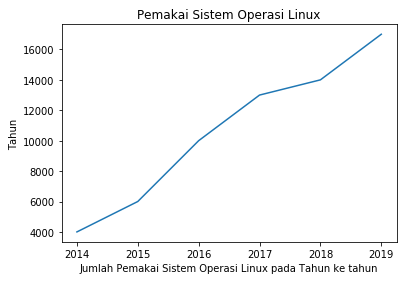
\includegraphics[width=12cm]{figures/6/1174042/7.png}
		\centering
		\caption{Hasil compile membuat diagram menggunakan Matplotlib.}
	\end{figure}
	
\end{enumerate}

\subsubsection{Soal No. 4}
\hfill \break
Jelaskan bagaimana cara menggunakan legend dan label serta kaitannya dengan fungsi tersebut!

\begin{enumerate}
	\item Untuk menggunakan legend definisikan parameter label di tiap fungsi plot. Parameter label digunakan untuk memberikan label pada line sebagai pembeda antar line.
	
	\lstinputlisting[caption = Kode program menggunakan parameter label dengan Matplotlib., firstline=123, lastline=124]{src/6/1174042/1174042.py}
	
	\item Kemudian panggil fungsi legend.
	
	\lstinputlisting[caption = Kode program memanggil fungsi legend dengan Matplotlib., firstline=128, lastline=128]{src/6/1174042/1174042.py}
\end{enumerate}

\hfill \break
\textbf{Kode Program}

\lstinputlisting[caption = Kode program membuat diagram menggunakan Matplotlib., firstline=117, lastline=130]{src/6/1174042/1174042.py}

\hfill \break
\textbf{Hasil Compile}

\begin{figure}[H]
	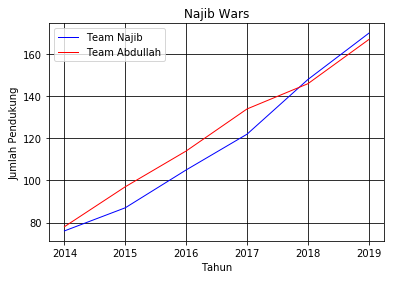
\includegraphics[width=12cm]{figures/6/1174042/8.png}
	\centering
	\caption{Hasil compile membuat diagram menggunakan Matplotlib.}
\end{figure}

\subsubsection{Soal No. 5}
\hfill \break
Jelaskan apa fungsi dari subplot di matplotlib, dan bagaimana cara kerja dari fungsi subplot, sertakan ilustrasi dan gambar sendiri dan apa parameternya jika ingin menggambar plot dengan 9 subplot di dalamnya!

\hfill \break
Fungsi subplot adalah untuk membuat beberapa plot di dalam satu gambar.
\hfill \break
Cara kerja subplot, yaitu fungsi subplot memiliki parameter pertama adalah jumlah kolom, parameter kedua adalah jumlah baris, dan parameter ketiga adalah index plot keberapanya.

\hfill \break
\textbf{Kode Program}

\lstinputlisting[caption = Kode program membuat subplot menggunakan Matplotlib., firstline=134, lastline=146]{src/6/1174042/1174042.py}

\hfill \break
\textbf{Hasil Compile}

\begin{figure}[H]
	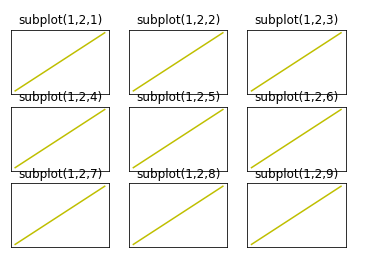
\includegraphics[width=12cm]{figures/6/1174042/9.png}
	\centering
	\caption{Hasil compile membuat subplot menggunakan Matplotlib.}
\end{figure}

\subsubsection{Soal No. 6}
\hfill \break
Sebutkan semua parameter color yang bisa digunakan (contoh:  m,c,r,k,...  dkk)!

\begin{itemize}
	\item 'b' (blue)
	\item 'g' (green)
	\item 'r' (red)
	\item 'c' (cyan)
	\item 'm' (magenta)
	\item 'y' (yellow)
	\item 'k' (black)
	\item 'w' (white)
\end{itemize}

\subsubsection{Soal No. 7}
\hfill \break
Jelaskan bagaimana cara kerja dari fungsi hist, sertakan ilustrasi dan gambar sendiri!

\hfill \break
Cara kerja dari fungsi hist yaitu fungsi hist akan menerima parameter yang diberikan, kemudian fungsi hist akan dieksekusi sesuai dengan parameter yang diberikan.

\hfill \break
\textbf{Kode Program}

\lstinputlisting[caption = Kode program membuat diagram menggunakan Matplotlib., firstline=150, lastline=157]{src/6/1174042/1174042.py}

\hfill \break
\textbf{Hasil Compile}

\begin{figure}[H]
	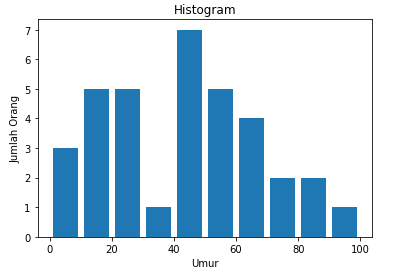
\includegraphics[width=12cm]{figures/6/1174042/10.png}
	\centering
	\caption{Hasil compile membuat diagram menggunakan Matplotlib.}
\end{figure}

\subsubsection{Soal No. 8}
\hfill \break
 Jelaskan lebih mendalam tentang parameter dari fungsi pie diantaranya labels, colors, startangle, shadow, explode, autopct!
 
 \begin{itemize}
 	\item labels : untuk memberikan label di tiap persentase.
 	\item colors : untuk memberikan warna di tiap persentase.
 	\item startangle : untuk memutar plot sesuai dengan derajat yang ditentukan.
 	\item shadow : untuk memberikan bayangan pada plot.
 	\item explode : untuk memisahkan antar tiap potongan pie pada plot.
 	\item autopct : untuk menentukan jumlah angka dibelakang koma.
 \end{itemize}

\subsection{Plagiarisme}
Berikut hasil pengecekan plagiarisme untuk bagian teori.
\begin{figure}[H]
	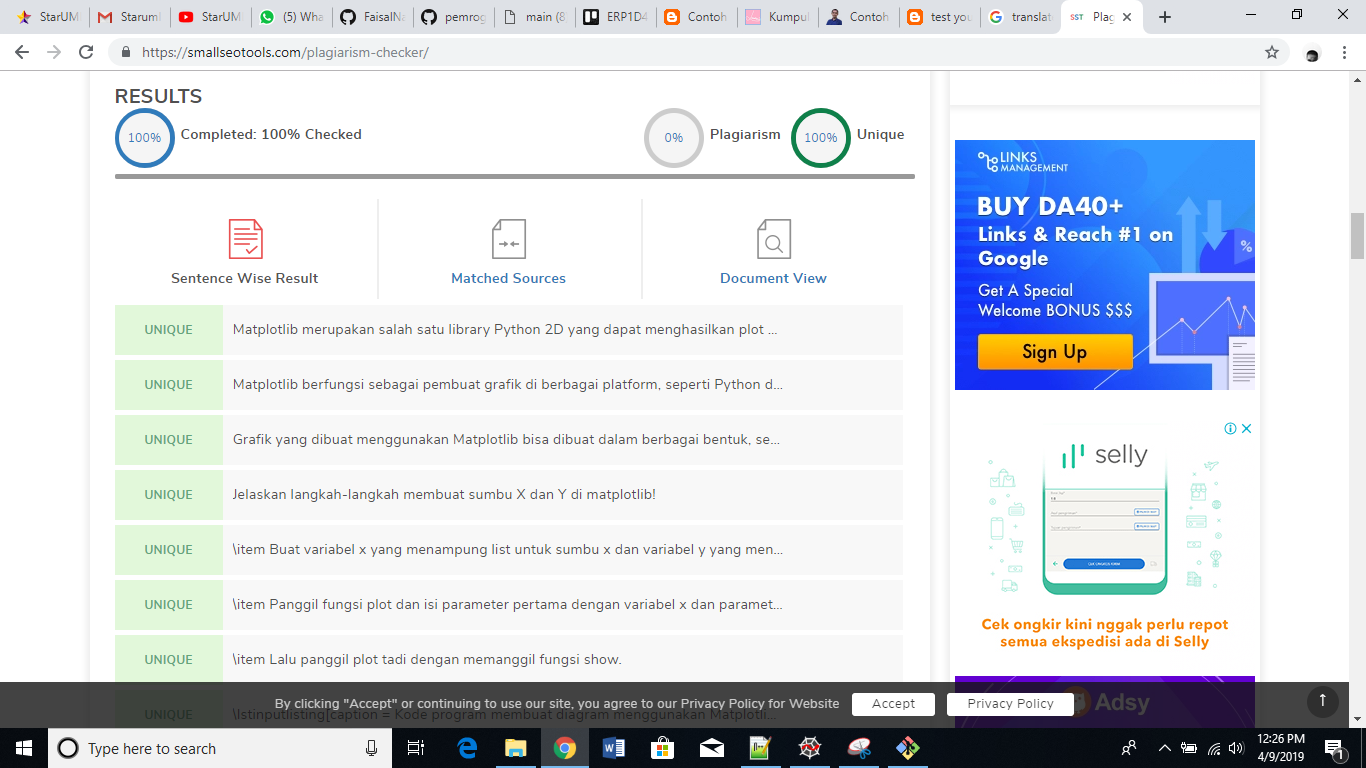
\includegraphics[width=12cm]{figures/6/1174042/plagiat.png}
	\centering
	\caption{Plagiarisme}
\end{figure}